% -----
% ARQUIVO: capitulo-03.tex
% VERSÃO: 1.1
% DATA: Janeiro de 2016
%
% CAPÍTULO DE CONCEITOS BÁSICOS DA PROPOSTA
%
% NÃO MEXA NAS SEÇÕES, SOMENTE EDITE O CONTEÚDO.
% -----

\chapter{Fundamentação Teórica e Estado da Arte}
% #TXT_CONCEITOS
\textcolor{RedOrange}{Divide-se em seções e subseções que variam em função da abordagem do tema. Deve iniciar com a Fundamentação Teórica que servirá de base para o desenvolvimento da dissertação. Os conceitos importantes devem ser claramene definidos, os quais devem ser levantados em artigos publicados (em periódicos e conferências relevantes da área de pesquisa) e em livros consolidados.}

\textcolor{RedOrange}{Segue o Estado da Arte, conforme o tema do trabalho desenvolvido, o qual deve ser pesquisado em bases de dados de artigos (Web of Science, Scopus, Science Direct, Scielo entre outras), preferencialmente artigos atuais (últimos 5-10 anos), em periódicos e conferências reconhecidos na área. Deve conter a exposição ordenada do assunto -- ordem cronológica dos trabalhos, procurando mostrar a evolução do tema, com as devidas citações (referências) -- evidenciando que existem questões em aberto e que há interesse na comunidade em resolver o problema (relevância e complexidade do problema).}

Mauris tempor ligula sed lacus. Duis cursus enim ut augue. Cras ac magna. Cras nulla. Nulla egestas. Curabitur a leo. Quisque egestas wisi eget nunc. Nam feugiat lacus vel est. Curabitur consectetuer \citep{Araujo2015}. Gini eect on Secondary school enrollment Lorem ipsum dolor sit amet, consectetuer adipiscing elit. Ut purus elit, vestibulum ut, placerat ac, adipiscing vitae, felis. Curabitur dictum gravida mauris. Nam arcu libero, nonummy eget, consectetuer id, vulputate a, magna \citep{Folha2015}. Donec vehicula augue eu neque.


% Para usar figuras, use sempre o mesmo template abaixo. altere somente:
% 1. os parâmetros do comando \includegraphics[width=•]{•} / tamanho e arquivo
% 2. \caption{*} / para colocar o rótulo da figura em *
% 3. \label{*} / para colocar a chamada para a figura no texto em *
%    TODA figura deve ter uma chamada no texto e esta deve ser feita sempre no formato:
%    Figura \ref{•} (p. ex. "Figura \ref{fig:artigo1}")

\begin{figure}[!h]
	\centering
	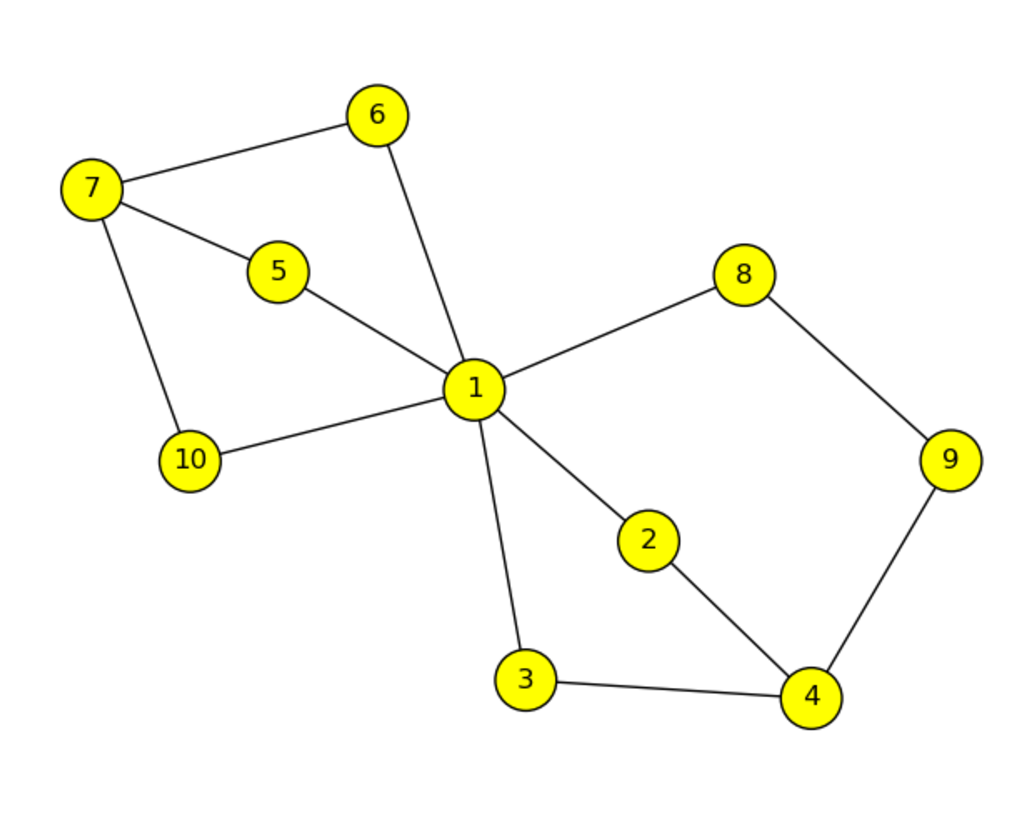
\includegraphics[width=0.4\textwidth]{artigo1.eps}
	\caption{R\'{o}tulo da Figura 1, descrevendo a figura.}
	\label{fig:artigo1}
\end{figure}

Pellentesque habitant morbi tristique senectus et netus et malesuada fames ac turpis egestas, como se pode ver na Figura \ref{fig:artigo1}. Mauris ut leo. Integer sapien est, iaculis in, pretium quis, viverra ac, nunc. Praesent eget sem vel leo ultrices bibendum. Aenean faucibus. Morbi dolor nulla, malesuada eu, pulvinar at, mollis ac, nulla. Sed ut perspiciatis unde omnis iste natus error sit voluptatem accusantium doloremque laudantium, totam rem aperiam, eaque ipsa quae ab illo inventore veritatis et quasi architecto beatae vitae dicta sunt explicabo.

%
% Ambiente de teoremas: \begin{*}
% * pode assumir os seguinte valores:
%	1. thm  - Teorema (na sequência, o texto aparece em itálico)
%	2. prop - Proposição
%	3. defn - Definição (na sequência, o texto aparece em itálico)
%	4. exmp - Exemplo
%	5. nota - Nota
%
\begin{thm}
Um Teorema simples:
\begin{equation}
X^2 := x^2 - 123
\label{thm1}
\end{equation}
\end{thm}

\lipsum[13] 

%
% Referência para um teorema (é igual para todas as opções do ambiente de teoremas)
Conforme o Teorema \ref{thm1}, nemo enim ipsam voluptatem quia voluptas sit aspernatur aut odit aut fugit, sed quia consequuntur magni dolores eos qui ratione voluptatem sequi nesciunt. Neque porro quisquam est, qui dolorem ipsum quia dolor sit amet, consectetur, adipisci velit, sed quia non numquam eius modi tempora incidunt ut labore et dolore magnam aliquam quaerat voluptatem. Ut enim ad minima veniam, quis nostrum exercitationem ullam corporis suscipit laboriosam, nisi ut aliquid ex ea commodi consequatur? Quis autem vel eum iure reprehenderit qui in ea voluptate velit esse quam nihil molestiae consequatur, vel illum qui dolorem eum fugiat quo voluptas nulla pariatur?


